%-shell-escape, якщо використовуєте minted
\documentclass[a4paper, 12pt, oneside]{extarticle}
\input{$HOME/Templates/lpnu_doc_templates/settings/preamble.tex}
% якщо домахуються за Times New Roman, то
% використовуєте xelatex і цей файл:
\input{$HOME/Templates/lpnu_doc_templates/settings/font_styles.tex}
\input{$HOME/Templates/lpnu_doc_templates/settings/minted_settings.tex}

\newcommand\Variant{4}
\newcommand\Date{24.04.\the\year}
\newcommand\Discipline{Алгоритмізація та програмування, частина 2}
\newcommand\Instructor{Кулешник Я. Ф.}
\usepackage{float}

\newcommand\Type{\Lab}
\newcommand\Number{11}
\newcommand\Topic{Теорія графів}

\usepackage{graphviz}

\begin{document}
\Margins

\Margins
%\begin{wrapfigure}[3]{l}{.27\textwidth}
%\includegraphics[width=.28\textwidth]{$UNI/.templates/lpnu_logo.png}
%\end{wrapfigure}

%\noindent\textbf{Прізвище:} \Lname \\
%\noindent\textbf{Ім'я:} \Fname \\
%\noindent\textbf{Група:} \Group \\
%\noindent\textbf{Варіант:} \Variant \\
%\noindent\textbf{Дата захисту:} \Date \\
%\\
%\noindent\textbf{Кафедра:} \Department \\
%\noindent\textbf{Дисципліна:} \Discipline \\
%\noindent\textbf{Перевірив:} \Instructor \\

%%\medskip\bigskip

%\begin{center}
%	\textbf{ЗВІТ}		\\
%	до \Type~\No\Number	\\
%	на тему ``\Topic''	\\
%\end{center}

% \begin{table}
%   \begin{tabularx}{\textwidth}{|c|X|X|}
%     \hline
%     % Image & Content & Additional Info \\
%     % \hline
% 	  \multirow{3}{*}{\includegraphics[width=4cm]{$UNI/.templates/lpnu_logo.png}}
% 	  & \textbf{ЗВО:}
% 	  Національний університет ``Львівська Політехніка''.
% 	  & \textbf{Тема:}
% 	  \Topic
% 	  \\
% 	  & \textbf{Навчальний рік:}
% 	  2023/2024
% 	  & \textbf{Інститут}
% 	  комп'ютерних наук та інформаційних технологій
% 	  \\
% 	  & \textbf{Семестр:}
% 	  осінній
% 	  & \textbf{Група:}
% 	  \Group
% 	  \\
% 	  & \textbf{Навчальна дисципліна:}
% 	  \Discipline
% 	  & \textbf{Студент:}
% 	  Мілюхін Олександр
% 	  \\
% 	  & \textbf{Кафедра}
% 	  систем автоматизованого проектування
% 	  &
% 	  \\
% 	  & \textbf{Викладач:}
% 	  Чумакевич В. В.
% 	  &
% 	  \\
%     \hline
%   \end{tabularx}
% \end{table}

\setlength{\textfloatsep}{-16pt}
% \setlength{\intextsep}{0pt}

\begin{table}
	\begin{tabular}{|l|l|p{6cm}|}
    \hline
    % Image & Content & Additional Info \\
    % \hline
	  \makecell[l]{
	  \includegraphics[width=3.37cm]{$UNI/.templates/lpnu_logo.png}
  }
	  & \makecell[l]{
	  \textbf{ЗВО:}
	  Національний університет \\ ``Львівська Політехніка''.
	  \\
	  \textbf{Навчальний рік:}
	  2023/2024
	  \\
	  \textbf{Семестр:}
	  осінній
	  \\
	  \textbf{Навчальна дисципліна:} \\
	  \Discipline
	  \\
	  \textbf{Кафедра}
	  систем автоматизованого \\ проектування
	  \\
	  \textbf{Викладач:}
	  Чумакевич В. В.
}
	  & \makecell [l] {
	  \textbf{Тема:}
	  \Topic
	  \\
          \textbf{Інститут}
	  комп'ютерних наук та \\ інформаційних технологій
	  \\
	  \textbf{Група:}
	  \Group
	  \\
	  \textbf{Студент:}
	  Мілюхін Олександр
  }
  \\
    \hline
  \end{tabular}
\end{table}
\section{Мета роботи}

% \begin{table}
%   \begin{tabularx}{\textwidth}{|p{6cm}|c|c|}
% 	  \hline
%     \multirow{3}{*}{\includegraphics[width=6cm]{$UNI/.templates/lpnu_logo.png}}
% 	  & ЗВО: Національний університет ``Львівська Політехніка''
% 	  & Additional Info 1 \\
%     & Content 2 & Additional Info 2 \\
%     & Content 3 & Additional Info 3 \\
% 	  \hline
%   \end{tabularx}
% \end{table}

% \begin{table}
%   \begin{tabular}{|c|c|c|}
%     \hline
%     \multirow{3}{*}{\includegraphics[width=3cm]{$UNI/.templates/lpnu_logo.png}} & \makecell{Content 1 \\ Content 2 \\ Content 3} & \makecell{Additional Info 1 \\ Additional Info 2 \\ Additional Info 3} \\
%     \hline
%   \end{tabular}
% \end{table}


вивчити основні визначення та правила використання
теорії графів, правила побудови матриць суміжності та інцидентності.

\section*{Індивідуальне завдання}

Згідно з варіантом побудувати граф на основі карти даної області України,
вершинами позначити районні центри, ваги ребра позначати за формулою
відстань = відстань в сантиметрах помножити на коефіцієнт масштабу.
Відстань перевести у кілометри, побудувати матрицю суміжності, матрицю
інцидентності.

\textbf{4 Дніпропетровська область}

\section*{Етапи розв'язку}

Для початку я ввів позначення для міст.

\begin{table}[h]
	\centering
	\begin{tabular}{c|c}
		Kr & Кривий Ріг \\
		Ka & Кам'янське \\
		Ni & Нікополь \\
		No & Новомосковськ \\
		Dn & Дніпро \\
		Sy & Синельникове \\
		Pa & Павлоград \\
	\end{tabular}
	\caption{позначення вершин}
\end{table}

\begin{figure}[h]
	\centering
	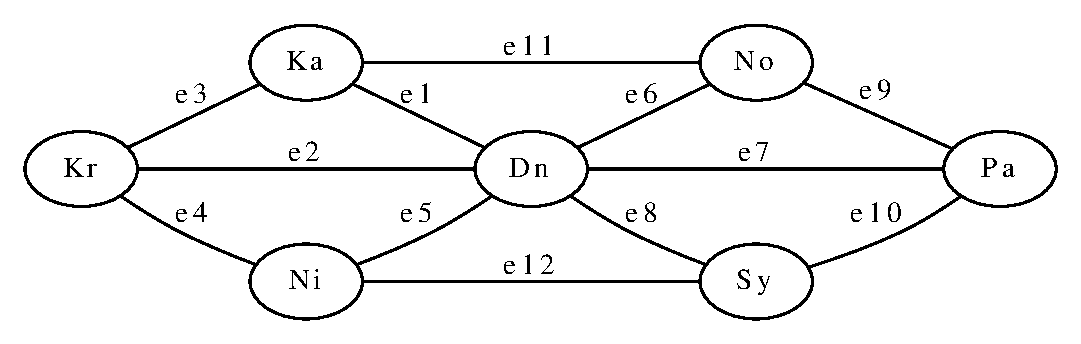
\includegraphics[width=.7\textwidth]{edges}
	\caption{Граф із позначеннями ребер}
\end{figure}

\begin{table}[h]
	\centering
	\begin{tabular}{c|c|c|c|c|c|c|c|c|c|c|c|c}
		&e1	&e2	&e3	&e4	&e5	&e6	&e7	&e8	&e9	&e10	&e11	&e12 \\
		\hline
		Kr &	&1	&1	&1	&	&	&	&	&	&	&	&\\
		\hline
		Ka &1	&	&1	&	&	&	&	&	&	&	&1	& \\
		\hline
		Ni &	&	&	&1	&1	&	&	&	&	&	&	&1 \\
		\hline
		No &	&	&	&	&	&1	&	&	&1	&	&1	& \\
		\hline
		Dn &1	&	&	&	&1	&1	&	&1	&	&	&	& \\
		\hline
		Sy &	&	&	&	&	&	&	&1	&	&1	&	&1 \\
		\hline
		Pa &	&	&	&	&	&	&1	&	&1	&1	&	& \\
	\end{tabular}
	\caption{Матриця інцидентності}
\end{table}


Далі побудував граф, установивши потрібні значення для ребер.

\begin{figure}[h]
	\centering
	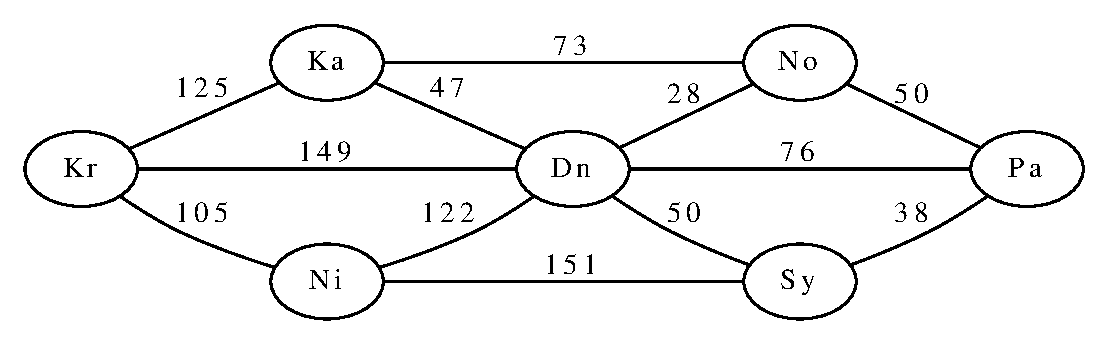
\includegraphics[width=.7\textwidth]{graph}
	\caption{Остаточний граф}
\end{figure}

\begin{table}[H]
	\centering
	\begin{tabular}{c|c|c|c|c|c|c|c }
		& Kr & Ka & Ni & No & Dn & Sy & Pa \\
		\hline
		Kr & 0 & 125 & 105 & 0 & 149 & 0 & 0 \\
		\hline
		Ka & 125 & 0 & 0 & 73 & 47 & 0 & 0 \\
		\hline
		Ni & 105 & 0 & 0 & 0 & 122 & 151 & 0 \\
		\hline
		No & 0 & 73 & 0 & 0 & 28 & 0 & 50 \\
		\hline
		Dn & 149 & 47 & 122 & 28 & 0 & 50 & 76 \\
		\hline
		Sy & 0 & 0 & 151 & 0 & 50 & 0 & 38 \\
		\hline
		Pa & 0 & 0 & 0 & 50 & 76 & 38 & 0 \\
	\end{tabular}
	\caption{Матриця суміжності}
\end{table}

\section*{Висновок}

У цій лабораторній роботі я пригадав те, що вивчив минулого семестру
на курсі дискретної математики та застосував новий для себе спосіб побудови графів.

\clearpage

\section*{Відповіді на контрольні запитання}
\begin{itemize}
	\question Що таке граф?
	\answer Множина вершин, з'єднаних ребрами.

	\question Чим цикл відрізняється від дерева?
	\answer Цикл --- замкнутий ланцюг, а в дереві всі ланцюги незамкнуті.

	\question Що таке неорієнтований граф?
		\answer граф, що містить тільки ребра (не дуги).

	\question Для чого використовують матрицю інцидентності?
	\answer Для передання зв'язків між вершинами й ребрами чи дугами

	\question Що таке вага ребра?
	\answer Вага ребра графа - це числове значення, яке присвоюється кожному ребру графа, щоб показати його важливість або вартість. Може позначати відстань між точками або пропускну здатність.

	\question Чим відрізняється список суміжності від матриці суміжності?
	\answer Список суміжності задається як масив, де кожен
		елемент є списком вершин, суміжних до певної вершини.

	\question Умова існування графа?
	\answer Наявність множини вершин та множини ребер,
		що їх з'єднують.

	\question Що таке мультиграф?
	\answer Граф, у якому дозволяється наявність кількох ребер, що з'єднують ті самі вершини.

	\question Для чого використовують графи?
	\answer Для моделювання зв'язків між об'єктами, зокрема
		транспортних та комунікаційних мереж, представлення
		статистичних даних.
\end{itemize}

\end{document}
